\subsection{Sprint 4}

Nesta \textit{sprint} final, assumi a responsabilidade de aprimorar o mapa com foco específico no Tecnopuc. O \ac{ages} IV Alessandro Borges de Souza estabeleceu contato direto com a equipe do parque tecnológico e, surpreendentemente, descobrimos que eles estavam iniciando um projeto com objetivos similares ao nosso. Essa coincidência abriu portas para uma colaboração: a equipe do Tecnopuc se comprometeu a fornecer uma amostra de empresas de cada prédio do parque, além de compartilhar um mapa desenvolvido na mesma biblioteca que utilizávamos.

Com base nessas informações, coordenei com os \ac{ages} II uma alteração estrutural importante na entidade dos expositores, adicionando o atributo ``prédio'' para armazenar a identificação do edifício correspondente. Essa modificação permitiu vincular adequadamente as empresas aos seus respectivos prédios.

Durante a primeira semana, Alessandro obteve o mapa prometido pela equipe do Tecnopuc. A qualidade do material recebido superou nossas expectativas, pois já continha todos os prédios modelados detalhadamente. Após análise, desenvolvi uma estratégia técnica: separar cada prédio em arquivos individuais e remontá-los em uma nova cena. Essa abordagem preservaria a funcionalidade essencial de destacar visualmente os prédios conforme as buscas realizadas pelos usuários. A Figura~\ref{fig:totem-tecnopuc-final} apresenta a versão final do mapa do Tecnopuc.

\begin{figure}[H]
    \centering
    \small
    \caption{Versão final do mapa do Tecnopuc}
    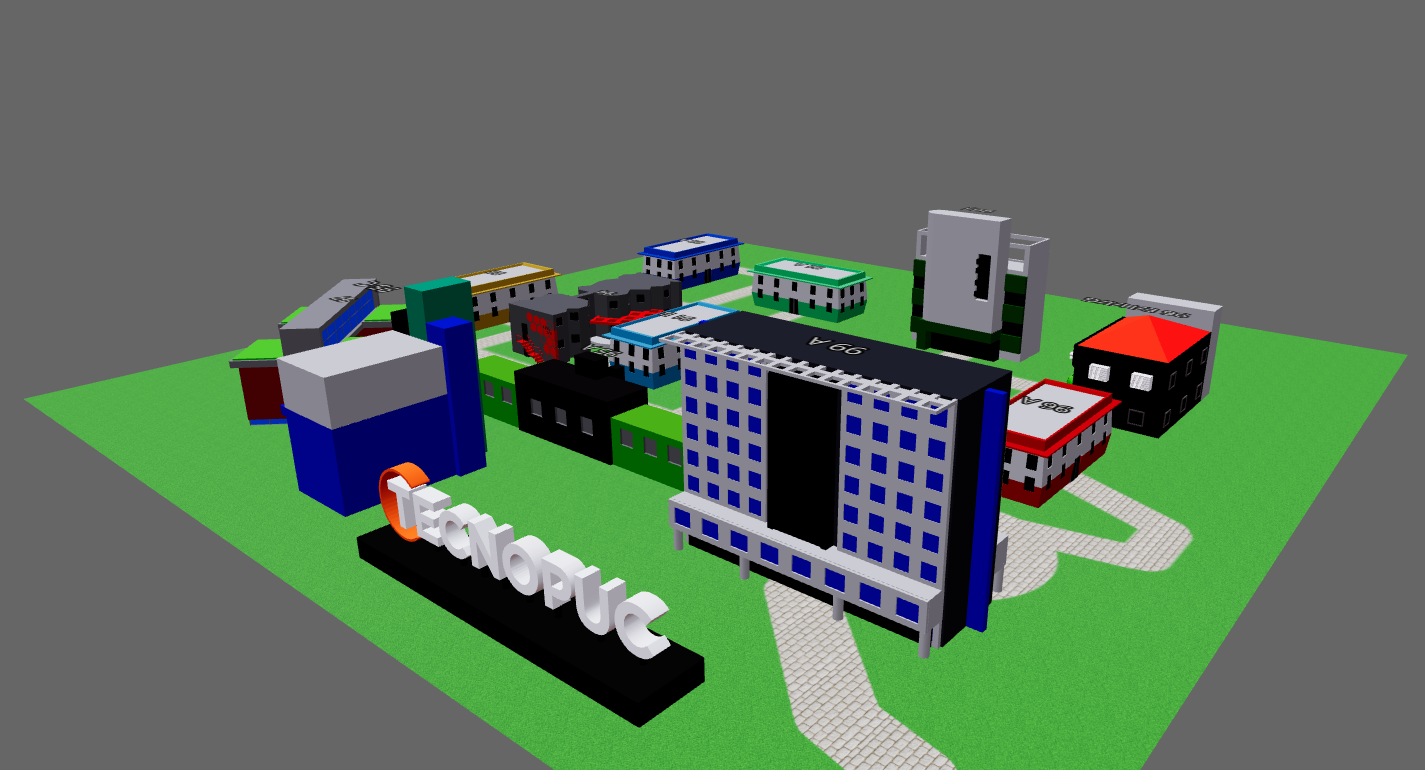
\includegraphics[width=0.9\linewidth]{conteudo/4 - ages III/images/fig10-mapa-tecnopuc-final.png}

    Fonte: Código-fonte do \textit{frontend}
    \label{fig:totem-tecnopuc-final}
\end{figure}

No \textit{backend}, a única funcionalidade pendente era aquela que havia ficado como débito técnico da \textit{sprint} anterior. Como estava sob responsabilidade de outro \ac{ages} III, optei por não intervir diretamente, confiando no processo estabelecido de acompanhamento.

Durante o desenvolvimento desta \textit{sprint}, observei um fenômeno preocupante: um relaxamento generalizado da equipe, incluindo os próprios \ac{ages} IV. O sucesso alcançado até então parecia ter criado uma falsa sensação de conclusão, quando na realidade diversos ajustes importantes ainda demandavam atenção. Essa situação resultou em acúmulo de tarefas para os momentos finais do projeto.

Na última semana, durante o \textit{code freeze}, identifiquei funcionalidades críticas do \textit{frontend} que permaneciam não implementadas, incluindo a integração do \textit{endpoint} de popular o banco com a página de administração. Em discussão com o \ac{ages} III Eduardo Felber Eichner, estabelecemos uma divisão: ele finalizaria a integração da tela de \textit{QR Code}, trabalho já iniciado na \textit{sprint} anterior, enquanto eu assumiria a integração do \textit{endpoint} de importação de dados.

A implementação transcorreu sem grandes obstáculos, pois a complexidade técnica era inferior aos desafios que havia enfrentado anteriormente. Desenvolvi uma tela intermediária, realizei a integração necessária e aguardei Eduardo concluir sua parte. Posteriormente, colaboramos na implementação do último elemento da interface administrativa: o botão de exportação de dados dos usuários e suas pesquisas no totem.

No dia da apresentação, dediquei-me a adicionar refinamentos que enriquecessem a experiência do usuário. Percebi que não havíamos implementado um método adequado para acessar a área administrativa. Solucionei essa lacuna criando um botão discreto que, ao ser acionado, exibia uma \textit{modal} solicitando senha de acesso ao painel administrativo.

Durante a validação final com os \ac{ages} IV, fui informado sobre um serviço \ac{aws} implementado para geração dinâmica de \textit{QR Codes} durante a apresentação. Nos testes, identifiquei uma incompatibilidade: o \textit{frontend} esperava \textit{QR Codes} com texto em português, enquanto o serviço gerava conteúdo em inglês. Rapidamente criei uma \textit{branch} específica para a apresentação e implementei a correção necessária, garantindo o funcionamento perfeito do sistema.

A apresentação final superou todas as expectativas. Além do \textit{stakeholder} Igor Daudt, contamos com a presença ilustre de Jorge Audy, um dos principais idealizadores do Tecnopuc. A demonstração não apenas impressionou nosso cliente original, mas despertou genuíno interesse do convidado especial. Jorge Audy compartilhou que o Tecnopuc enfrenta desafios significativos com a localização de auditórios, pois visitantes frequentemente se perdem entre os diversos prédios ao procurar salas de palestras.

Esta \textit{sprint} final consolidou o sucesso do projeto, transformando nossa solução em uma ferramenta com potencial real de aplicação. A validação por figuras importantes do ecossistema tecnológico confirmou a relevância e qualidade do trabalho desenvolvido. Apesar dos desafios enfrentados com o relaxamento da equipe e as correções de última hora, a capacidade de adaptação e resolução rápida de problemas garantiu uma entrega impecável, demonstrando a maturidade técnica alcançada ao longo do projeto.
